\documentclass{standalone}
\usepackage{tikz}

\usetikzlibrary{calc}

\begin{document}

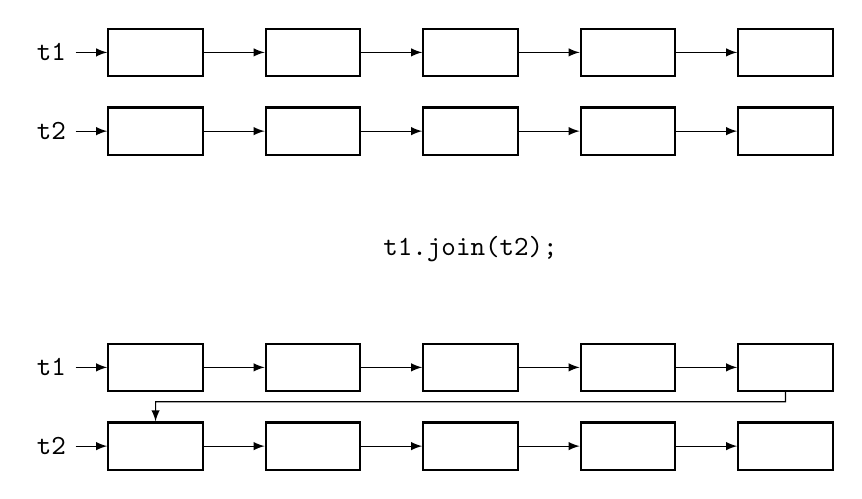
\begin{tikzpicture}[wagon/.style={minimum width=1.2cm,minimum height=0.6cm,draw,black,thick},
                    link/.style={-latex,thin},
                    address/.style={font=\tiny,circle,thin,fill=white}]

  \foreach[count=\i] \c in {20,30,25,55,5} {
    \pgfmathparse{(\i-1)*2}\let\x\pgfmathresult
    \node[wagon] (w\i) at (\x,0) {};
  }
  \foreach \i in {1,2,3,4} {
    \pgfmathparse{int(\i+1)}\let\j\pgfmathresult
    \draw[link] (w\i.east) -- (w\j.west);
  }

  \begin{scope}[yshift=-1cm]
    \foreach[count=\i] \c in {20,30,25,55,5} {
      \pgfmathparse{(\i-1)*2}\let\x\pgfmathresult
      \node[wagon] (ww\i) at (\x,0) {};
    }
    \foreach \i in {1,2,3,4} {
      \pgfmathparse{int(\i+1)}\let\j\pgfmathresult
      \draw[link] (ww\i.east) -- (ww\j.west);
    }
  \end{scope}

  \node[anchor=east] (var) at ($ (w1.west) + (-.4,0) $) {\tt t1};
  \draw[-latex] (var.east) -- (w1.west);

  \node[anchor=east] (var) at ($ (ww1.west) + (-.4,0) $) {\tt t2};
  \draw[-latex] (var.east) -- (ww1.west);




  \begin{scope}[yshift=-4cm]
    \foreach[count=\i] \c in {20,30,25,55,5} {
      \pgfmathparse{(\i-1)*2}\let\x\pgfmathresult
      \node[wagon] (v\i) at (\x,0) {};
    }
    \foreach \i in {1,2,3,4} {
      \pgfmathparse{int(\i+1)}\let\j\pgfmathresult
      \draw[link] (v\i.east) -- (v\j.west);
    }
  \end{scope}

  \begin{scope}[yshift=-5cm]
    \foreach[count=\i] \c in {20,30,25,55,5} {
      \pgfmathparse{(\i-1)*2}\let\x\pgfmathresult
      \node[wagon] (vv\i) at (\x,0) {};
    }
    \foreach \i in {1,2,3,4} {
      \pgfmathparse{int(\i+1)}\let\j\pgfmathresult
      \draw[link] (vv\i.east) -- (vv\j.west);
    }
  \end{scope}

  \node[anchor=east] (var) at ($ (v1.west) + (-.4,0) $) {\tt t1};
  \draw[-latex] (var.east) -- (v1.west);

  \node[anchor=east] (var) at ($ (vv1.west) + (-.4,0) $) {\tt t2};
  \draw[-latex] (var.east) -- (vv1.west);

  \draw[-latex] (v5.south) -- ($ (v5.south) ! .33 ! (vv5.north) $) -| (vv1.north);


  \node at ($ (v1.north west) ! .5 ! (ww5.south east) $) {\tt t1.join(t2);};
\end{tikzpicture}

\end{document}